\section{RL basics}
Firstly, an environment where an agent can operate must be defined. The environment can be described by Markov decision process (MDP), where $S_t \in \mathcal{S}$ is a state from a set of possible states $\mathcal{S}$ in which the environment could be located in time $t$. In the environments with the observable MDP, an agent can observe the state of the environment and make the action accordingly. An action is a probabilistic transition between the states. Every action $A_t \in \mathcal{A}$ moves the environment from $S_t$ to $S_{t+1}$. If we consider the lidar planning task, the action is sending the rays in certain direction and the state is given by the position of the sensor and by the already executed measurements. The environment evaluates every action and returns appropriate reward $R_t$ (see Figure \ref{fig:rlconcept}). In RL the set $\mathcal{A}$ is often called an action space and the set $\mathcal{S}$ an observation space. A return $G_t$ is a sum of the discounted future rewards \cite{sutton2012}.
\begin{equation}
G_t = \sum\limits_{k=0}^{\infty}\gamma^k R_{t+k}
\end{equation}
where $\gamma \in [0,1]$ is a discount factor. The RL methods define how experience from interacting with the environment will change the policy. The major issue is that maximizing of the immediate reward is often not an effective approach to maximize the sum of discounted rewards $G_t$. This greedy policy can take the agent into a very disadvantageous state. Thus, the agent must take into account the future states and rewards. The goal of the agent is to find policy $\pi$ which maximizes the expected return. The agent use the value function $V_{\pi}(S_t)$ which assesses how advantageous is being in the state $S_t$ with the policy $\pi$.
\begin{equation}
V_{\pi}(S_t) \doteq  \mathbf{E}_\pi[G_t | S_t].
\end{equation}
An optimal policy $\pi^*$ is then defined for all $S_t \in \mathcal{S}$ as
\begin{equation}
\pi^*(S_t) \doteq \max\limits_\pi V_\pi(S_t).
\end{equation}
In the past, agents used big tables to estimate the value function. That is possible in environments with small action and observation spaces but is very memory consuming for larger environments and even impossible for a continuous action or observation space. Therefore, the modern methods use neural networks as function estimators.

\begin{figure}[!h]
\centering
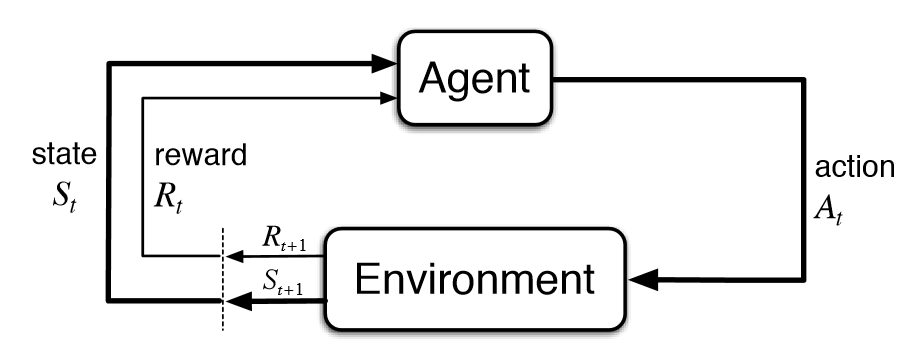
\includegraphics[scale=0.15]{fig/RL-concept.png}
\caption[RL concept]{Illustration of RL concept. Source - \cite{sutton2012}.}
\label{fig:rlconcept}
\end{figure}


\subsection{Temporal difference learning}
Temporal difference (TD) learning combines the ideas of Monte Carlo methods and the dynamic programming. It can learn directly from experience obtained by an interactions with the environment without any prior knowledge of the said environment. The TD learning is done by following assignment in each timestamp \cite{sutton2012}
\begin{align} \label{eq:TD}
\delta_t &= R_{t} + \gamma V(S_{t+1}) - V(S_t) \\
V(S_t) &\gets V(S_t) + \lambda \delta_t
\end{align}
where $\delta_t$ i the TD and $\lambda \in \mathbb{R}^+$ is step size.

\subsection{Q-learning}
Q-learning is a type of TD learning developed by Watkins \cite{watkins1992}. The state value $V$ from the previous subsection is replaced by the $Q$ value, which refers to a quality of action in a particular state instead of the quality of the state itself. When we rewrite the TD learning \eqref{eq:TD} to the Q-learning we get:
\begin{equation}
Q(S_t, A_t) \gets Q(S_t, A_t) + \lambda [R_{t} + \gamma \underset{A_{t+1}}{\max} Q(S_{t+1}, A_{t+1}) - Q(S_t, A_t)].
\end{equation}
The policy here is to take the action with the maximum $Q$ value. That is called the greedy policy. An obvious drawback of greedy policy is that it does not allow to explore the whole environment properly because an action with the highest $Q$ value is always chosen. A solution to this problem is to make sometimes a random action, and explore the environment. This policy is often referred to as the $\epsilon$-greedy policy.

\begin{algorithm}
\caption{$\epsilon$-greedy policy in pseudocode}
\begin{algorithmic}[1]
\Function{ChooseAction}{}
\State $\epsilon \gets \epsilon \cdot \epsilon_d$
\If {$\epsilon >$ random $\in (0,1)$}
\State action $\gets$ random $\in \mathcal{A}$
\Else 
\State action $\gets$ $\underset{A_t}{\max} Q(S_t, A_t)$
\EndIf
\State \Return action
\EndFunction
\end{algorithmic}
\end{algorithm}

It is common to set $\epsilon = 1$ at the beginning of the training and the decay rate $\epsilon_d$ close to one. The general idea behind this policy assumes that it is needed to explore the environment first and then exploit experience of the agent.

\clearpage

\subsection{Prioritized experience replay}
The prioritized experience replay is a biologically inspired mechanism introduced by Schaul et al. \cite{schaul2015} which stores all experience (specifically: $S_t$, $A_t$, $R_{t}$, $S_{t+1}$) in a buffer and assigns priority to every experience. The main idea is that experience with a high TD should have the higher priority. It is thus necessary to calculate the priority $p$ from the TD error:
\begin{equation}
p = (|\delta_t | + \eta)^\rho
\end{equation}
where $\rho$ indicates how much we prefer experience with the higher priority and $\eta \ll 1$ is a constant which helps to avoid the priorities very close to zero. Considering a greedy selection would abandon experience with the low priority, a better approach is to choose experience $i \in \mathcal{I}$ with the probability
\begin{equation}
P(i) = \frac{p_i}{\sum\limits_{j \in \mathcal{I}} p_j},
\end{equation}
where $\mathcal{I}$ is the set of all experience in the buffer. It is now possible to sample a batch of experience for training using this probability. It removes a correlation in the observation sequence and improves the sample efficiency of the DQN. It is feasible to store all the experience in a buffer sorted by the priority, but a more efficient implementation is a sum tree. That is a binary tree, where the value of each root is equal to the sum of its children values (see Figure \ref{fig:sumtree}). Example of the usage is in the algorithm \ref{alg:sumtree}.
\begin{algorithm}
\caption{Retrieve node from sum tree in pseudocode}
\label{alg:sumtree}
\begin{algorithmic}[1]
\Function{GetChild(parent, value)}{}
\If {parent.left is None} \Return parent \EndIf
\If {value $\leq$ parent.left.value} 
\State \Return GetChild(parent.left, value)
\Else 
\State \Return GetChild(parent.right, value - parent.left.value)
\EndIf
\EndFunction
\end{algorithmic}
\end{algorithm}
\begin{figure}[H]
\centering
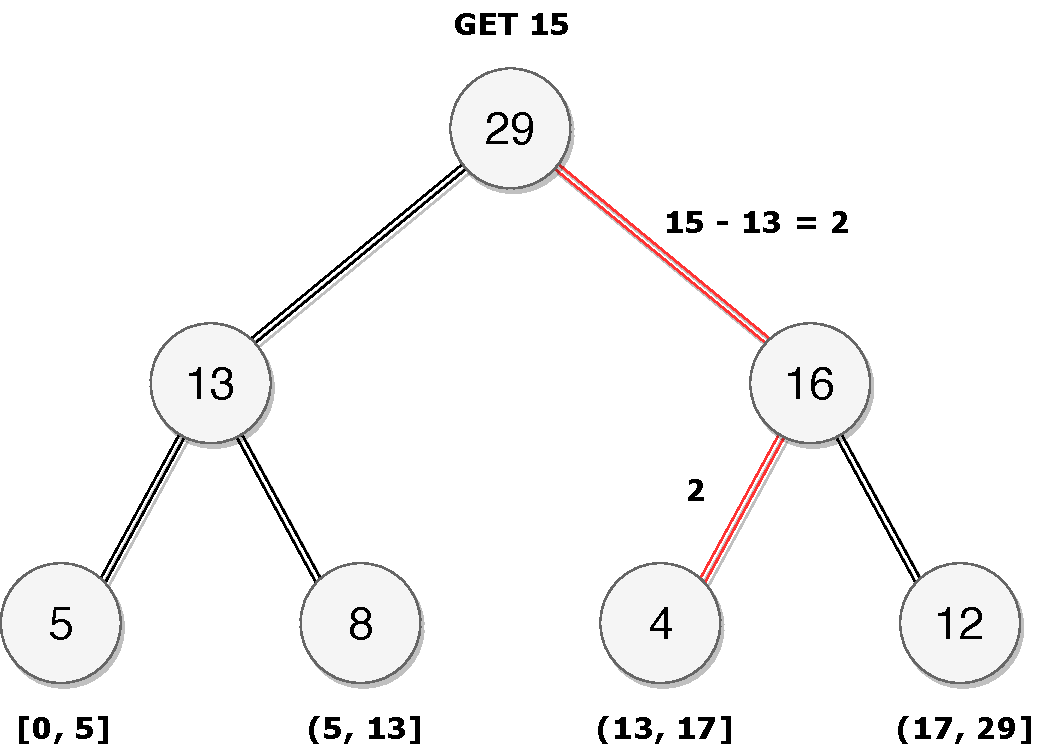
\includegraphics[scale=0.5]{fig/sumtree.pdf}
\caption[Sum tree]{Simple example of sum tree.}
\label{fig:sumtree}
\end{figure}
\clearpage
\section{Deep neural networks in RL}
As was stated in the previous chapter, the tabular methods are very inefficient in the large environments. In these cases, it is possible to use the deep neural networks which can replace the tables. Deep Q networks (DQN) proposed by Google Deepmind \cite{mnih2015} outperformed all previous RL algorithms in playing Atari games. With the neural networks also grew the popularity of policy gradient methods where function estimator outputs an action instead of Q values. Note that most of these methods are general and not necessarily tied to the neural networks.

\subsection{Deep Q network}
The neural network takes the current state as input and outputs the Q value for each possible action. The network is trained using gradients of the Q-value in the current state with respect to trainable weights $\theta$ of the neural network.
\begin{align} \label{eq:qlearn}
\delta_t &= R_{t} + \gamma \underset{A_{t+1}}{\max}Q^\theta(S_{t+1}, A_{t+1}) - Q^\theta(S_t, A_t)\\
\theta_{t+1} &= \theta_t + \lambda \delta_t \nabla_\theta Q^\theta (S_t, A_t).
\end{align}
The weights are updated in proportion to the TD $\delta_t$. Unfortunately, this simple DQN agent suffers from a lack of the sample efficiency and often does not converge well. There are many techniques which can help to the DQNs to achieve satisfying results.

\subsection{Target network}
Target network is a technique which improves the convergence of a DQN learning \cite{mnih2015}. It uses two neural nets instead of one. Firstly is trained online network on a batch of data and the target network is used for predictions during training. After the completion of the training on a batch of data, the target network is updated \cite{lilicrap2015}.
\begin{equation}
\theta^- = \tau \theta + (1-\tau)\theta^-,
\end{equation}
where $\theta^-$ is the set of trainable weights of the target network, $\theta$ indicates the weights of the online network and $\tau \ll 1$ is constant.
TD $\delta$ is now calculated using the target network:
\begin{equation}
\delta_t = R_{t} + \gamma \underset{A_{t+1}}{max}Q^{\theta^-}(S_{t+1}, A_{t+1}) - Q^\theta(S_t, A_t). 
\end{equation}
The target network stabilizes the training since the predicting network does not change after each training step.

\subsection{Double Q-learning}
Classic Q-learning algorithm tends to overestimate actions under certain conditions. Hasselt et al. propose the idea of a Double Q-learning which decompose the max operation into action selection and action evaluation \cite{hasselt2015}.The TD is then computed by the following equation.
\begin{equation}
\delta = R_{t} + \gamma Q^{\theta^-}(S_{t+1}, \underset{A_{t+1}}{\text{argmax}}Q^\theta(S_{t+1}, A_{t+1})) - Q^\theta (S_t, A_t).
\end{equation}
The double DQN outperforms the DQN in terms of the value accuracy and the policy quality.

\section{Policy gradient}
By this section, the goal of the neural network was predicting the values by which the policy was determined. In policy gradient methods the neural networks approximate the policy itself. 
\begin{align}
J = \mathbf{E}_\pi[G_t | S_t, A_t, \theta_t] \\
\theta_{t+1} = \theta_t + \lambda \widehat{\nabla_\theta J}
\end{align}
where $J$ is a performance measure with respect to our the neural network parameters and $\widehat{\nabla_{\theta} J}$ is a stochastic estimate of the gradient of the performance measure. In other words, this method is basically doing a stochastic gradient ascent of $J$ with respect to $\theta$ \cite{sutton1999}. The policy gradient methods are outperforming the DQNs, especially in the continuous action spaces, because it does not have to estimate the Q-value for every possible action.

\subsection{Actor-Critic}
Thanks to predicting the action directly, it is much easier to predict in the continuous action space, but the Q-value which assessed the quality of the action in the certain state has been lost. That is why the Actor-Critic framework was created. It uses two separate neural networks - actor which predicts the action and critic which assesses an advantage of the action. This concept is visualised in Figure \ref{fig:actorcritic}.
\begin{figure}[H]
\centering
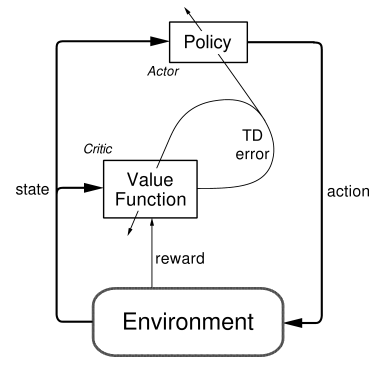
\includegraphics[scale=0.55]{fig/actor-critic.png}
\caption[Actor-Critic framework]{Actor-Critic framework. Source - \cite{sutton2012}.}
\label{fig:actorcritic}
\end{figure}

Consider the critic using the Q-values for an update. $\theta$ and $\omega$ denote the trainable weights of actor and critic, respectively. Critic update is similar to DQN:
\begin{align}
\delta_t &= r_t + \gamma Q^\omega(S_{t+1}, \mu ^\theta (S_{t+1})) - Q^\omega(S_t, A_t)\\
\omega_{t+1} &= \omega_t + \lambda \delta_t \nabla_\omega Q^\omega(S_t, A_t).
\end{align}
Note that instead of $A_{t+1}$ is now used function $\mu^\theta(S_{t+1})$, which is an action estimate by the neural network of the actor. The update rule of the actor is not so straightforward. 
\begin{equation}
\theta_{t+1} = \theta_t + \lambda\nabla_\theta \mu^\theta(S_t)\nabla_a Q^\omega (S_t, A_t)|_{a = \mu^\theta(S_t)}.
\end{equation}
This equation uses the chain rule for derivatives to obtain the gradient of Q-values with respect to the trainable weights $\theta$. Namely:
\begin{equation}
\frac{\partial Q^\omega(S_t, A_t)}{\partial \theta} = \frac{\partial Q^\omega(S_t, A_t)}{\partial A_t} \frac{\partial A_t}{\partial \theta}.
\end{equation}
The neural network of the actor is updated by gradients which change the action output to maximize the Q-value of the critic \cite{silver2014}.
There are other approaches, which doesn't use the Q-value as critic assessment, but they rather use so-called advantage \cite{schulman2017}. These methods are beyond the scope of this thesis. 
\clearpage
\subsection{Stochastic Actor-Critic}
A stochastic Actor-Critic method is a frequently used approach. In this method the actor outputs a parameters of a probability distribution and the action itself is sampled from the parameterized distribution. It is a standard to use a normal distribution and predict a mean and variance of the action. The biggest advantage of the normal distribution is that it can be adjusted to the use of a backpropagation \cite{hess2015}. Another benefit of the stochastic actor is that it does not need any other techniques for the action space exploration.

\subsubsection{Beta distribution}
On the other hand, an obvious drawback of the normal distribution is that there is always some small probability of sampling an outlier. There is also an issue for a bounded action space. When mean value of the normal distribution is close to the boundary, an agent can experience a not negligible bias. A solution for both problems is to use Beta distribution as the stochastic policy \cite{chou17}. The Beta distribution is defined by the following function:
\begin{equation}
f(x;\alpha, \beta) = \frac{\Gamma(\alpha + \beta)}{\Gamma(\alpha)\Gamma(\beta)}x^{\alpha-1}(1-x)^{\beta-1},
\end{equation}
where $\alpha,\beta \in R^+_0$ are the distribution parameters and $x \in [0, 1]$. $\Gamma$ is Euler's gamma function, which extends factorial into the set of real numbers. The Beta distribution is shown in Figure \ref{fig:beta}. The biggest advantage is that Beta distribution is bounded by definition and does not need any additional clipping.

\begin{figure}[H]
\centering
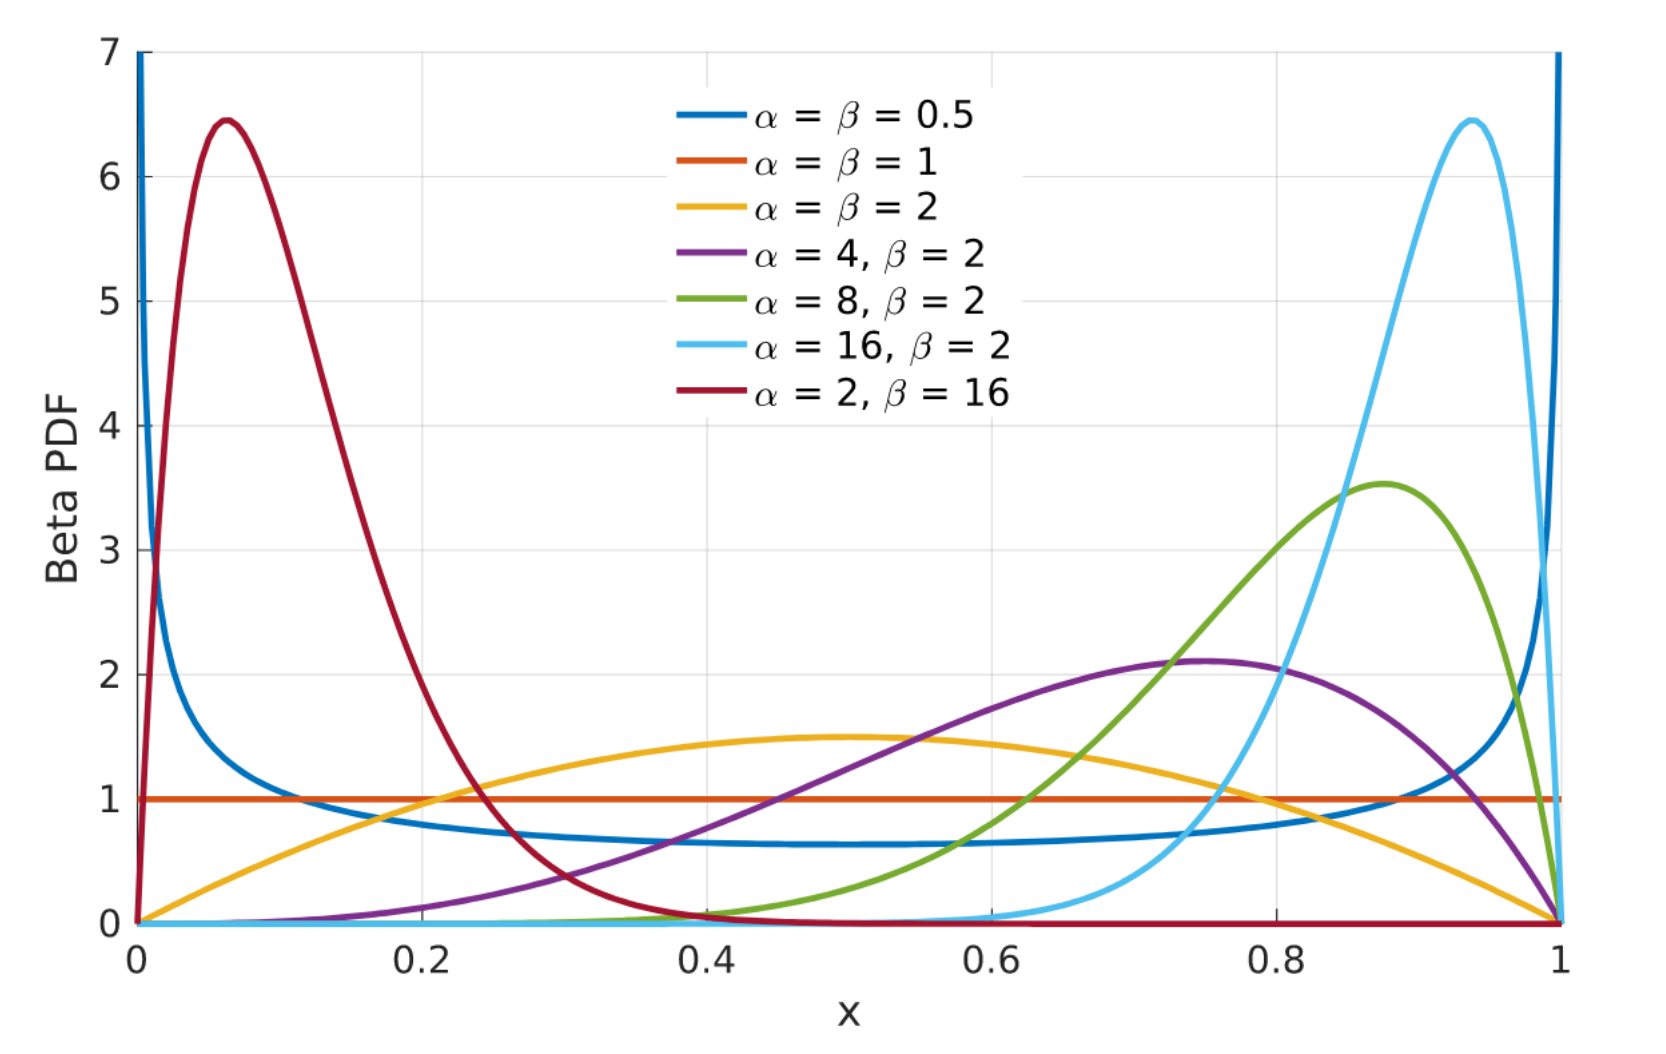
\includegraphics[scale=0.2]{fig/beta.png}
\caption[Probability density of beta distribution]{Probability density of beta distribution. Source - \cite{chou17}.}
\label{fig:beta}
\end{figure}

For the reinforcement learning is suitable only $\alpha, \beta \geq 1$. That makes the Beta distribution concave and unimodal. This can be ensured by using a softplus activation and adding one at the end of actor-network.

\subsection{Deterministic policy gradients}
Deep deterministic policy gradient (DDPG) is one of the methods for exploiting the Actor-Critic framework. Whereas the stochastic actor predicts the distribution parameters and samples an action, the DDPG outputs the action directly. Silver \cite{silver2014} has shown that the deterministic policy can outperform its stochastic counterparts. A disadvantage of a deterministic approach is that it needs an additional policy to ensure the action space exploration. The exploration methods are discussed in the subsection \ref{sec:exploration}.

\subsection{Parameter and action space noise}
\label{sec:exploration}
In the large action space is crucial to emphasize an exploration of the agent. Wrong exploration can cause that the agent converges prematurely and ends up in a local optimum. The DDPG commonly uses the stochastic policy to slightly modify actions of the actor.
\begin{equation} \label{eq:exploration}
\hat{A_t} = \mu^\theta(S_t) + \mathcal{N}(0, \sigma^2)
\end{equation}
where $\mathcal{N}$ is the normal distribution with the mean value equal to zero and the variance, which is reducing during the training. $\hat{A_t}$ is a perturbed action. An action space noise helps the agent to explore the environment. \par Another approach is to apply the noise directly to the weights of the neural network of the actor. It can sometimes lead to more consistent exploration and richer behaviors \cite{plappert2017}.
\begin{equation}
\hat{\theta} = \theta + \mathcal{N}(0, \sigma^2)
\end{equation}
where the policy using $\hat{\theta}$ is a so-called perturbed actor, which is interacting with the environment. 
\clearpage
The major issue of the parameter space noise is that it is much harder to tune. When we use the action space noise, it is easier to estimate its impact on the actions (differences between both approaches can be seen in Figure \ref{fig:exploration}). Because of an unpredictable influence of the parameter space noise is necessary to use an adaptive noise scaling.
\begin{align}
d &= |\mu^{\hat{\theta}}(S_t) - \mu^\theta(S_t)|_2  \\
\sigma_{t+1} &= 
     \begin{cases}
       \kappa \sigma_t & \text{if } d \leq T \\
       \frac{1}{\kappa}\sigma_t & \text{otherwise}
     \end{cases}
\end{align}
where $\kappa$ is a scaling factor slightly bigger than one and $T$ is a threshold value, which has to be tuned to the specific environment.
\par When it is necessary to explore the action space near to some desired action or include a momentum of the environment, it is possible to use Ornstein-Uhlenbeck random process \citep{lilicrap2015}, 
\begin{equation}
\hat{A_t} = \mu^\theta(S_t)  + \nu (\rho - \mu^\theta(S_t)) + \phi \mathcal{N}(0, 1),
\end{equation}
where $\nu, \phi \in [0, 1]$ are constants of the random process and $\rho$ is mean value around which we want to explore the action space. When $\nu = 0$ it is a basic exploration as in the expression \eqref{eq:exploration}.

\begin{figure}[H]
\centering
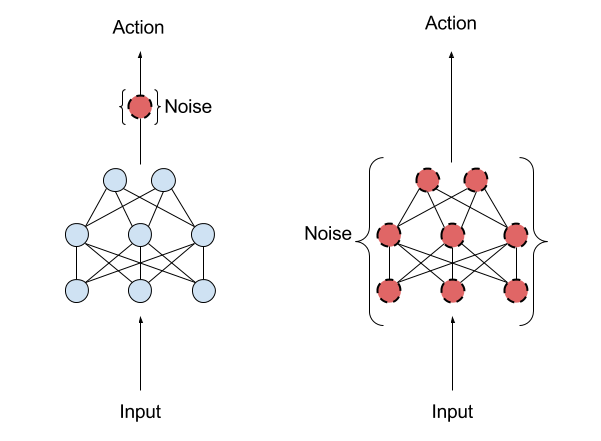
\includegraphics[scale=0.5]{fig/perturbations.png}
\caption[Exploration noise types]{Left - action space noise, Right - parameter space noise. Source - \cite{plappert2017}.}
\label{fig:exploration}
\end{figure}